\section{Blockchain Search Engine}
\label{sec:search}

\subsection{Introduction}

As an increasing number of smart contracts are deployed by developers, searching needs for massive smart contracts soar. Given that smart contracts are simply code and include no functional descriptions, indexing smart contracts with search engine technologies imposes a high difficulty. To index smart contracts properly, we use the following methods:

%随着越来越多的智能合约被开发者部署,用户面对海量的智能合约,搜索的需求也变得突出起来。智能合约仅仅是代码,并不包含任何功能描述,很难利用搜索引擎技术为智能合约建立索引。我们将用多种手段为智能合约建立合适的索引:

\begin{itemize}
	\item Crawl webpage data relevant to smart contracts to set up mappings between the data and blockchain smart contracts.
	%\item 爬取智能合约相关网页资料,为其和区块链智能合约建立映射关系;
	\item Encourage developers to upload verified source code of smart contracts, analyze the functions and semantics of the code, create indexes for the source code, and provide the searching function for similar contracts. For smart contracts without source code, decompile them for their source code.
	%\item 鼓励开发者上传验证过的智能合约源代码,分析其代码功能和语义,为源代码建立索引,提供相似合约搜索;未提供源代码的智能合约,进行反编译得到其源代码;
	\item Establish standards for smart contracts so that any contracts matching those standards can be retrieved and found by users. Also, encourage developers to provide informational descriptions of contracts during smart contract creation.
	%\item 为智能合约建立规范,任何符合此规范的智能合约,都能被检索并被用户搜索到,鼓励开发者在创建智能合约时,提供合约信息描述。 \\

	\begin{figure}[ht]
  	\centering
  	\begin{minipage}{.4\linewidth}
	\begin{lstlisting}[frame=single]
contract SearchableContract {
   string public language;
   string public author;
   string public name;
   string public title;
   string public description;
   string public tags;
}
	\end{lstlisting}
  	\end{minipage}
	\end{figure}

\end{itemize}

\subsection{Infrastructure}

We believe that the centralized architecture is more suitable for obtaining the best user experience of the searching service. The Nebulas development team is dedicated to developing a searching service, retrieving all smart contracts in real time, performing multilingual word breaking and creating full-text indexes to provide users with a user-friendly web interface. The impartiality of the NR ranking algorithm and the verifiability of each node ensure the impartiality of the centralized searching service, while the complete code of the searching backend is available to the community. Also, third-party developers can create their own searching services on this basis. \reffig{fig:search-arch} shows the architecture of the searching service.

%我们认为,搜索服务为了提供最佳的用户体验,中心化的架构更为适合。星云链开发组将实现一个搜索服务,实时检索所有智能合约,做多语言的分词,建立全文索引,最终提供一个友好的Web界面给用户使用。\textbf{NR排名算法的公正性和每个节点的可验证性保证了中心化搜索服务的公正性},所有搜索后台代码都将开源给社区。第三方开发者也可据此创建独立的搜索服务。搜索服务架构如图\ref{fig:search-arch}所示。

\begin{figure}[h]
\centering
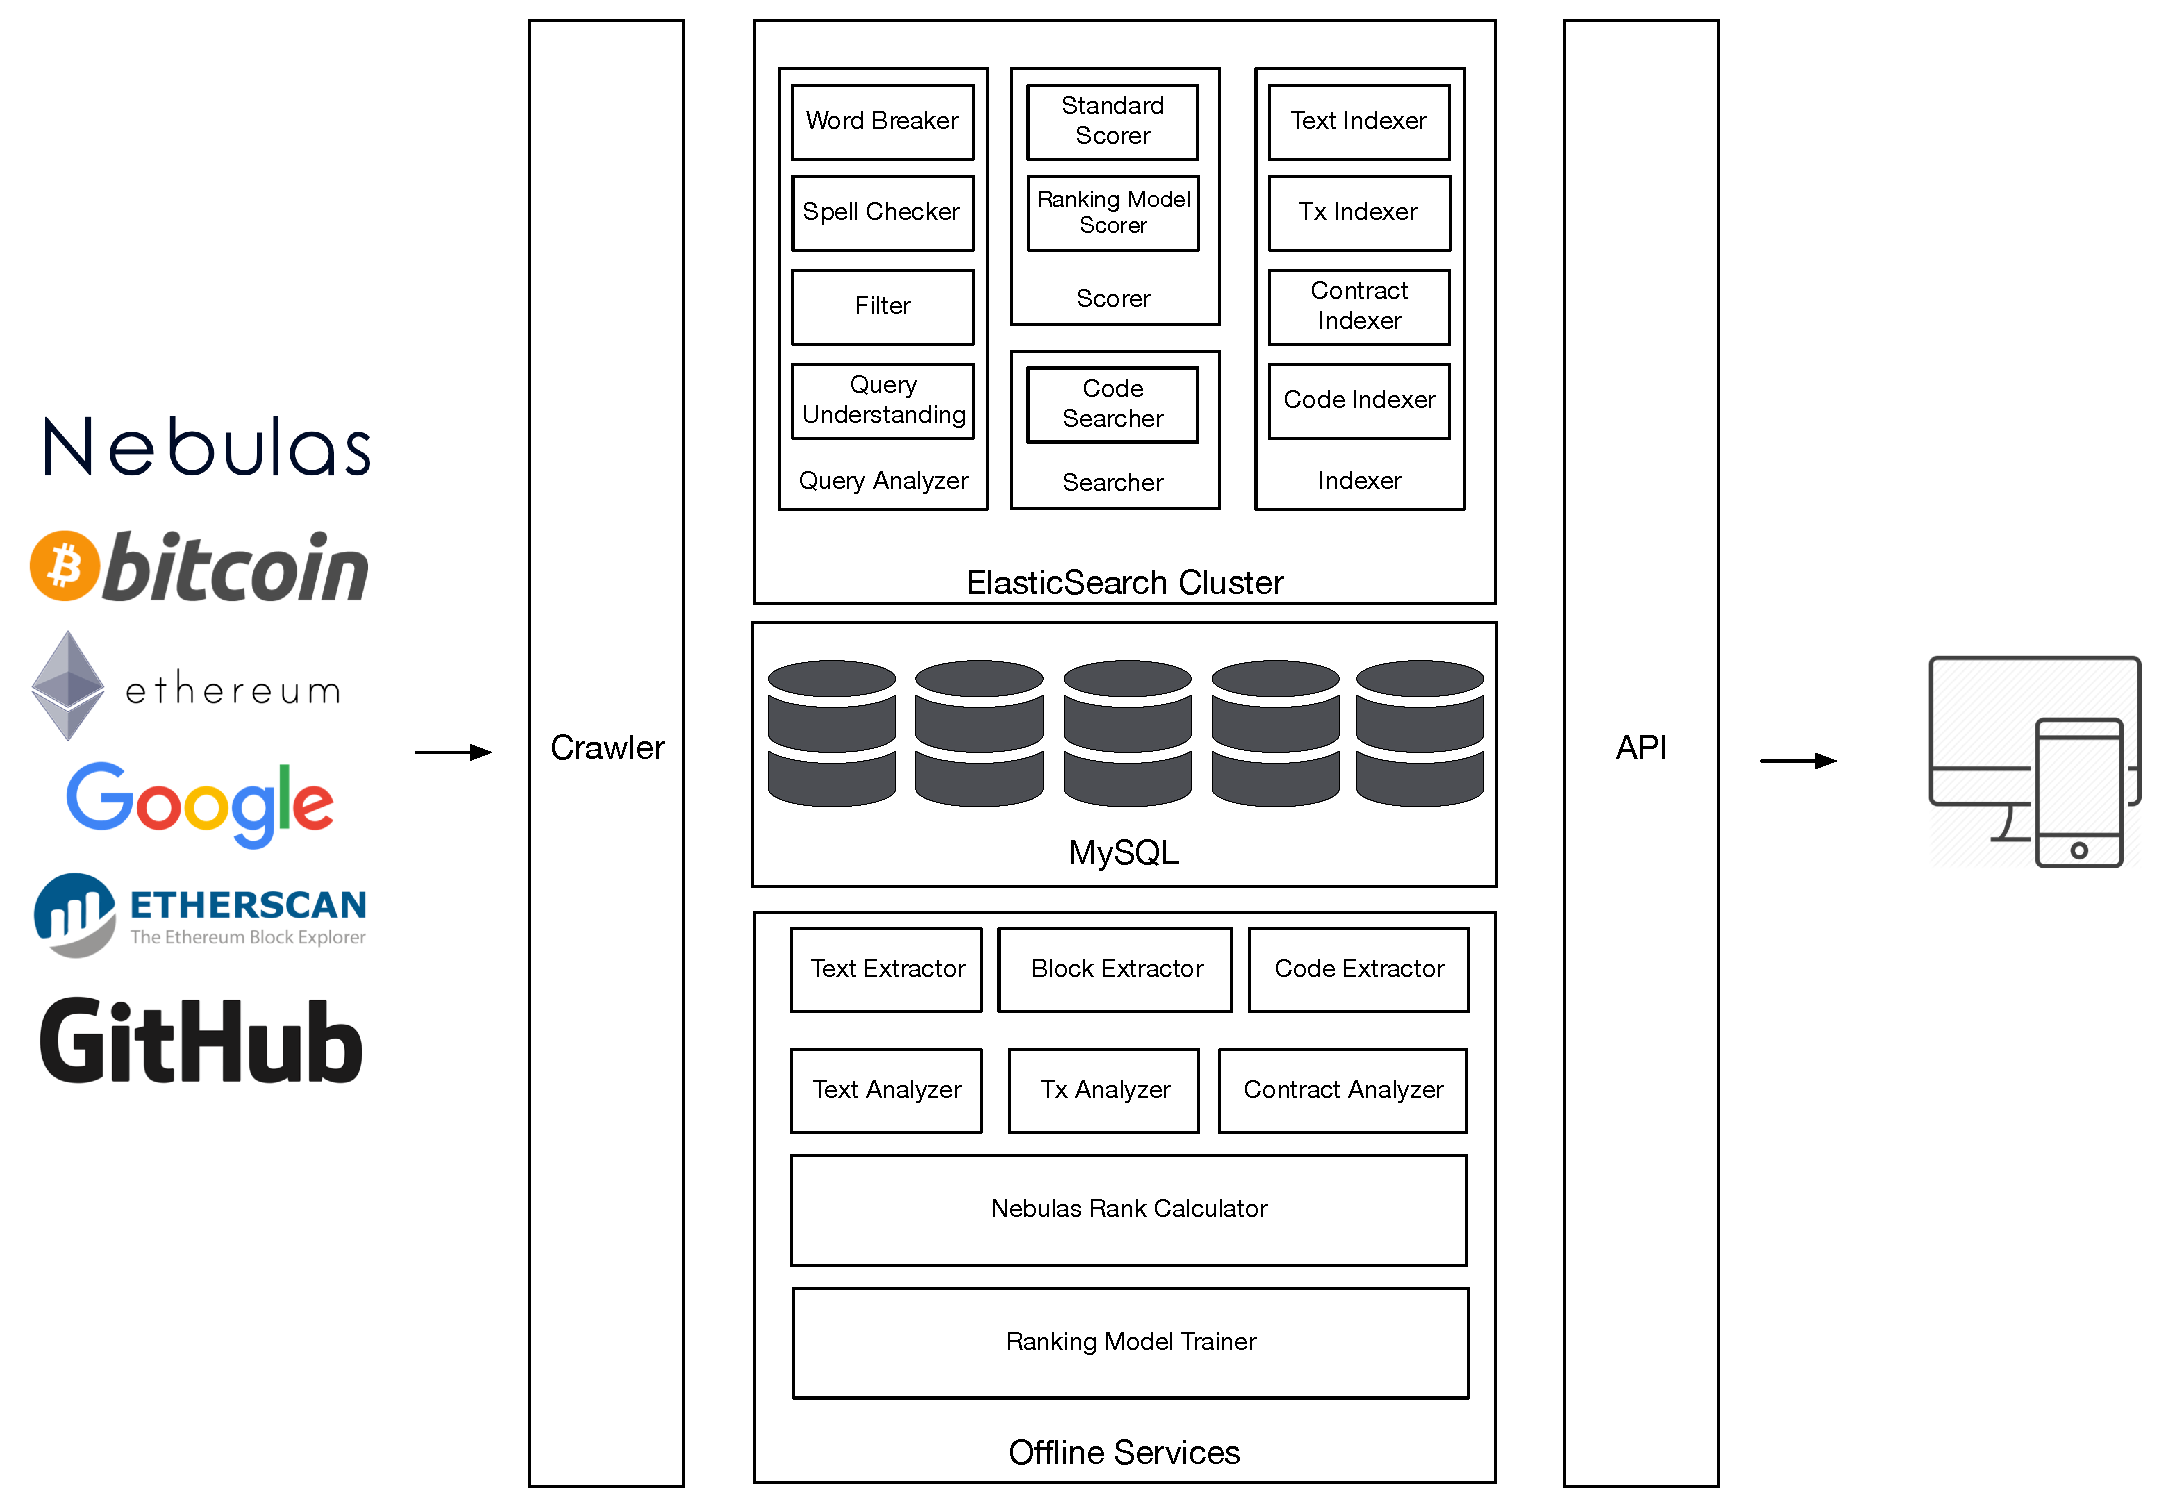
\includegraphics[width=16cm]{./figs/search-arch-new}
\caption{Architecture of the searching service}
\label{fig:search-arch}
\end{figure}

\begin{itemize}
	\item \textbf{Crawler}  Crawler data sources of the Crawler blockchain search engine are classified into two types: one for collecting block information and code of smart contracts from blockchains, while the other for crawling data about smart contracts from public URLs including introductions, Dapp user comments and news.
	%\item \textbf{Crawler} 区块链搜索引擎爬虫数据源分为两种,一种从区块链上收集区块信息和智能合约代码等信息,一种从公开网址上爬取智能合约相关资料,包括介绍、Dapp用户评论、新闻资讯等。
	\item \textbf{Extractor} consists of Text Extractor, Block Extractor and Code Extractor, which provide text information, block information and code extraction service for smart contracts, respectively.
	%\item \textbf{Extractor} 包括Text Extractor, Block Extractor和Code Extractor,分别提供文本信息、区块信息和智能合约代码提取服务。
	\item \textbf{Analyzer} consists of Text Analyzer, Tx Analyzer and Contract Analyzer, which are text information, block transaction information and smart contract analyzers, respectively. For the smart contract analyzer, it provides contract decompilation, source code extraction, semantic analysis and webpage parsing functions.
	%\item \textbf{Analyzer} 包括Text Analyzer, Tx Analyzer, Contract Analyzer,分别为文本信息、区块交易信息和智能合约分析器,其中智能合约分析器包括合约反编译、源代码功能、语义分析,网页解析等。
	\item \textbf{Nebulas Rank Calculator} refers to the Nebulas Rank calculator service, which is used to calculate the Nebulas Ranks of each non-contracted and contracted accounts offline.
	%\item \textbf{Nebulas Rank Calculator} 星云指数计算服务,离线计算每个非合约账户和合约账户的星云指数。
	\item \textbf{Ranking Model Trainer} refers to the ranking model trainer service. For transaction graph purposes, ranking rules take multiple factors into account: matching field, text relevance, NR Rank value of the contract, transaction quantity of the contract, frequency and depth, NR Rank of the user conducting a transaction with the contract, and contract security. Based on users' actual use conditions, the machine learning algorithm (GBDT and artificial neural network (ANN) are optional) is used to train the ranking and scoring model, which is also constantly improved according to user feedback. The trained model is used by Scorer of the searching service.
	%\item \textbf{Ranking Model Trainer} 排序模型训练。考虑到交易Graph,排序规则考虑了多个因素:匹配字段,文本相关度,合约的NR Rank值,合约的交易数量、频度和深度,与合约发生交易的用户NR Rank值,合约安全性等等。我们根据用户的实际使用情况,用机器学习算法(GBDT、人工神经网络都是候选)训练排序打分模型,根据用户的反馈不断优化。训练后的模型被搜索服务的Scorer使用。
	\item \textbf{Query Analyzer} refers to the keyword analysis service, which includes the multilingual word breaker (Word Breaker) and the spell checker (Spell Checker).
	%\item \textbf{Query Analyzer} 关键词分析服务,包括多语言分词器Word Breaker,拼写检查器Spell Checker等。
	\item \textbf{Indexer} creates proper indexes from Analyzer and supports both full and incremental indexing.
	%\item \textbf{Indexer} 从Analyzer中建立合适的索引,支持全量和增量索引。
	\item \textbf{Scorer} is classified into two levels: Level-1 Standard Scorer recalls candidate result sets from ElasticSearch, which is done to recall as many candidate results as possible through the efficient and effective ranking in the ElasticSearch cluster. Level-1 can recall several thousands of results. Level-2 Ranking Model Scorer uses the offline rank model to calculate and reorder the rank of each Level-1 candidate result set. For this level, the calculated results feature a sounding accuracy and can be used directly by users.
	%\item \textbf{Scorer} 分为两个level:Level-1 Standard Scorer从ElasticSearch中召回候选结果集,目标是尽可能把潜在的候选结果,在ElasticSearch集群中通过快速有效的排序打分召回,Level-1召回的结果数量有限,控制在几千以内;Level-2 Ranking Model Scorer使用 Offline Rank Model,计算每个Level-1结果候选集的得分,重新排序,这个结果较为精确,可以直接给用户使用。
	\item \textbf{Searcher} is responsible for communicating with the ElasticSearch cluster and packing and returning the search result to the searching frontend.
	%\item \textbf{Searcher} 负责和ElasticSearch集群通信,以及对搜索结果包装返回给搜索前端。
	\item \textbf{API} provides external applications with comprehensive searching API services.
	%\item \textbf{API} 对外提供完善的搜索API服务。
	\item \textbf{ElasticSearch Cluster} ES refers to the server cluster. The Nebulas development team plans to use the open-source search engine ElasticSearch to support full-text indexing.
	%\item \textbf{ElasticSearch Cluster} ES服务器集群。星云链团队考虑使用开源搜索引擎ElasticSearch作为其全文索引支持。
\end{itemize}

\subsection{Nebulas Trends}

The Nebulas creates the tendency list in combination with Nebulas Rank to provide user visual blockchains with multi-dimensional values.
%星云链将结合星云指数构建趋势榜单,提供给用户可视化的区块链多维度价值。

\begin{itemize}
\item \textbf{Nebulas Rank list for non-contracted accounts.} It displays the daily NR list and the NR quick rise and drop lists. Also, this rank list visualizes the rank variation tendency of each account and the health change tendency of the entire network.
%\item \textbf{非合约账户Nebulas Rank榜单}~~呈现每日NR榜单,以及NR快速提升和快速下降榜单,并且可视化呈现各个账户的R变化趋势,以及整个网络健康程度变化趋势。
\item \textbf{Nebulas Rank list for contracted accounts.} Based on the NR values of non-contracted accounts, the Nebulas Rank list calculates the NR list of contracted accounts, the quick rise and drop lists, the variation tendency of each contract and the tendency chart for the quantity and use frequency of smart contracts on the entire network. In addition, we will present other smart contract lists such as the token contract list and the market contract estimation list to display a wider dimension of information.
%\item \textbf{合约账户Nebulas Rank榜单}~~根据非合约账户NR值,计算合约账户的NR榜单,以及快速提升和快速下降榜单,各个合约的变化趋势,以及整个网络智能合约数量和使用频次的趋势图。除此之外,我们还将呈现不同领域的智能合约榜单,比如Token合约榜单、预测市场合约榜单等等,以展示更多维度的信息。
\item \textbf{Smart contract developer list.} According to the contracted account list, the list of smart contract developers calculates the contribution list of contracted developers and the contribution quick rise list to display outstanding contracted developers and their apps.
%\item \textbf{智能合约开发者榜单}~~根据合约账户榜单,计算合约开发者的贡献度榜单,以及贡献度快速提升榜单,展示优秀合约开发者及其应用。
\end{itemize}

\subsection{Keyword Query}

By providing a keyword or describing the textual information about a smart contract such as its title, author or function, users can find the matching contract from massive smart contracts. Currently, mature and sophisticated algorithms and technologies are available for text searching. By using the natural language processing and inverted index technologies, we can retrieve and sort efficiently in the index database for massive smart contracts. This involves the following key technologies:

%用户提供关键词,描述智能合约的标题、作者、功能等文本信息,在海量的智能合约中找到匹配的合约。对于文本搜索,目前有非常成熟的算法和技术,基于自然语言处理和倒排索引技术,我们可以在海量的智能合约索引库里高效的检索和排序。关键的技术如下:

\begin{enumerate}
	\item Topic-oriented distributed crawler technology
	\item Multilingual word breaking technology: word breaking is relatively simple for western words. For the word breaking of Chinese words, these algorithms are available: positive maximum matching, negative maximum matching, shortest path word breaking and statistical word breaking.
	\item Search term correction and semantic comprehension
	\item Inverted index and distributed searching architecture
	\item Ranking algorithm to sort the search results

	%\item 面向主题的分布式爬虫技术
	%\item 多语言分词技术:对于西文词汇,分词较为简单。对于中文分词,有多种算法可进行分词:正向最大匹配,逆向最大匹配,最短路径分词,统计分词等;
	%\item 查询词纠错、语义理解
	%\item 倒排索引,分布式搜索架构
	%\item 排序算法,给搜索结果排序
\end{enumerate}

Among these technologies, the ranking algorithm will be designed in combination with Nebulas Rank. Specifically, we use intra-user transfers in the blockchain world as an analogy to webpage reference relations in the Internet world to create the blockchain transaction graph. Then, calculate the NR rank of non-contracted users by using the NR ranking algorithm described in Section 2.3, calculate the ranks of those contracts by using the contract ranking algorithm described in Section 4.2, and lastly use the calculation result for search result sorting.

%其中排序算法将结合Nebulas Rank来设计,我们把区块链世界中用户之间的转账类比互联网世界的网页引用关系,构建出区块链交易图,然后利用\ref{subsec:leaderrank}中提出的NR排名算法,计算非合约用户的NR排名,然后结合\ref{dip:arith}中介绍的合约排名算法,计算合约的排名结果,最后应用于搜索结果排序。


\subsection{Searching for Similar Smart Contracts}

For developers and certain users, they may want to search for smart contracts with similar functions according to the code fragment of a contract. Being different from regular keyword searching, code similarity has its particularity. To implement the searching function for similar smart contracts, we need to use a certain algorithm to measure the code similarity in a number or percentage.

%开发者和某些用户,可能有根据合约代码片段,搜索具有相似功能的智能合约的需求。不同于普通的关键词搜索,代码相似度有其特殊性。我们需要有一定的算法,通过数值或者百分比的形式对代码相似度进行度量,从而提供相似智能合约搜索的功能。

In today's academia, code similarity algorithms are mainly categorized into the string edit distance, token sequence similarity, abstract syntax tree similarity and program dependency graph similarity. These algorithms describe the similarity in terms of code text, structure and syntax from different dimensions. By combining these 4 major algorithms, we put forward 12 characteristics of the code similarity of Nebulas contracts, such as Skeleton Tree, Type Signature and Library Calls. For details, see Appendix \ref{appendix:sim_code}.

%目前学术界对代码相似度算法主要有字符串编辑距离、Token序列相似度、抽象语法树相似度和程序依赖图相似度四个流派,他们分别从不同维度描述了代码文本、结构和语法上的相似度,我们结合主流4个流派的思路,提出了星云链合约代码相似度算法的12种特征,如Skeleton Tree、Type Signature和Libaray Calls等,详情见附录\ref{appendix:sim_code}。

Similar to search results of keywords, search results of smart contracts also use the same contract ranking algorithm to produce final results.

%相似智能合约搜索结果,和关键词搜索结果一样,使用同样的合约排名算法排序,给出最终结果。
